%%%%%%%%%%%%%%%%%%%%%%%%%%%%%%%%%% NAME %%%%%%%%%%%%%%%%%%%%%%%%%%%%%
%%%%%%%%%%%%%%%%%
\section{Complementary Filter}
%%%%%%%%%%%%%%%%%
%%%%%%%%%%%%%%%%%
\subsection{Angle Measurement}
\begin{frame}{Complementary Filter}{Angle Measurement}
	\begin{figure}
		\centering
		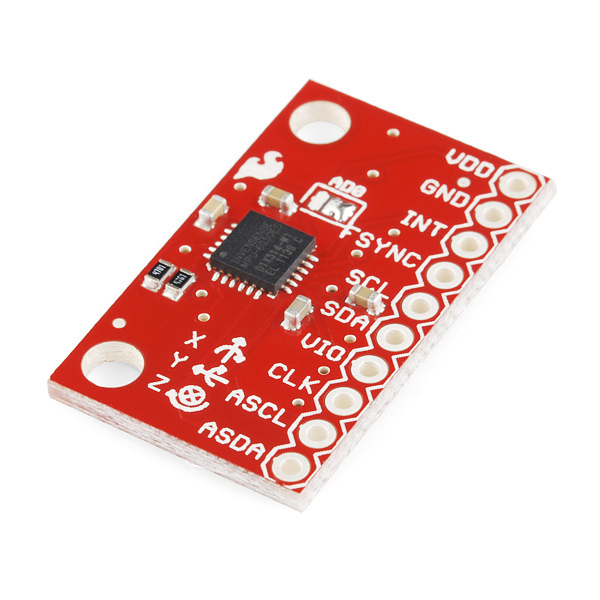
\includegraphics[scale=1.2]{Pictures/IMU6050.jpg}
	\end{figure}
\end{frame}
%%%%%%%%%%%%%%%%
%%%%%%%%%%%%%%%%
\subsection{Gyroscope}
\begin{frame}{Complementary Filter}{Gyroscope}
%A gyroscope measures angular velocity by integrating small intervals to find the orientations.
\begin{figure}
	\centering
	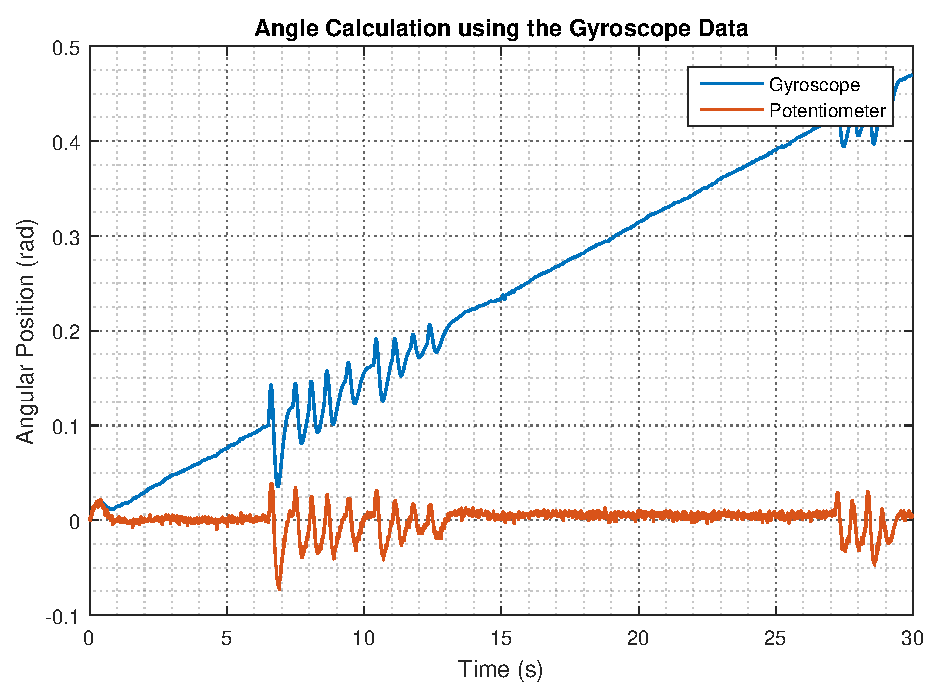
\includegraphics[scale=0.6]{Pictures/angleGyro.pdf}
\end{figure}
%
%The problems with the gyroscope are:
%	\begin{itemize}
%		\item {By integrating, the error is accumulating over time.}
%		\item {The gyroscope may experiencing drifting errors from small and slow movement.}
%	\end{itemize}
\end{frame}
%%%%%%%%%%%%%%%
%%%%%%%%%%%%%%%%
\subsection{Accelerometers}
\begin{frame}{Complementary Filter}{Accelerometers}
%An accelerometer measures inertial force, such as gravity and relies on a constant gravitational pull with respect to the Earth, and the calculations orientation can be found.
\begin{figure}
	\centering
	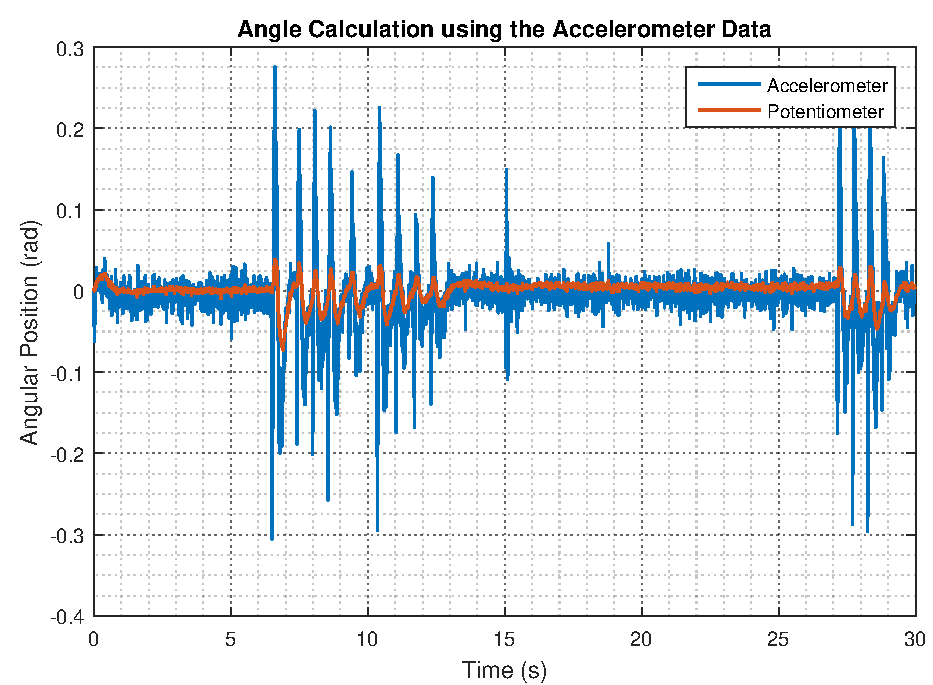
\includegraphics[scale=0.6]{Pictures/angleAcc.pdf}
\end{figure}
%
%The problems for accelerometers are:
%\begin{itemize}
%	\item {They are very sensitive to mechanical noise and vibrations.}
%\end{itemize}
\end{frame}
%%%%%%%%%%%%%%%%
%%%%%%%%%%%%%%%%
\subsection{Sensor Fusion}
\begin{frame}{Complementary Filter}{Sensor Fusion}
%Data from accelerometers and gyroscopes can be combined for a better estimate of orientation than using only accelerometer data.\linebreak
%
%The combined data can help fix noise and drift error. A method is to use a complementary filter.
\begin{figure}
	\centering
	\begin{tikzpicture}[ auto,
thick,                         %<--setting line style
node distance=2cm,             %<--setting default node distance
scale=0.9,                     %<--|these two scale the whole thing
every node/.style={scale=0.9}, %<  |(always change both)
>=triangle 45 ]                %<--sets the arrowtype
\draw%--------------------------------------------------------------------------------------------

node[shape=coordinate][](acc) at (0,0){acc}			% start of acc signal path

node[shape=coordinate][](acc1) at (2.5,0){acc1}

node(lowpas) at (6,0) [block] {\Large $\ \frac{1}{\tau \cdot s + 1}$ }

node[shape=coordinate][](gyro) at (0,-2){}		% start of gyro signal path

node(integrate) at (3,-2) [block] {\Large $\frac{1}{s}$}

node(highpas) at (6,-2) [block] {\Large $\ \frac{\tau \cdot s}{\tau \cdot s + 1}$ }

node(sum) at (8,-1) [sum] {$\sum$}


node[shape=coordinate][](angle) at (11,-1){}		% output of the complementary filter
;

\draw[-](acc) -- node {accel$\_\theta_{F}$} (acc1);
\draw[->](acc) -- node {} (lowpas);
\draw[->](gyro) -- node {gyro$\_\dot{\theta}_{F}$} (integrate);
\draw[->](integrate) -- node {} (highpas);

\draw[->](highpas) -| node {} (sum);
\draw[->](lowpas) -| node {} (sum);


\draw[->](sum) -- node {$\theta_{F}$} (angle);

\end{tikzpicture}

\end{figure}
%Complementary filter advantages is:
%\begin{itemize}
%	\item {Fast estimates of angle and much less lag than low-pass filter alone.}
%	\item {Not very processor-intensive.}
%\end{itemize}
\end{frame}
%%%%%%%%%%%%%%%%
%%%%%%%%%%%%%%%%
\subsection{Cut-off Frequency}
\begin{frame}{Complementary Filter}{Cut-off Frequency}
%High pass and low pass filters with the same cut-off frequency. 
\begin{figure}
	\centering
	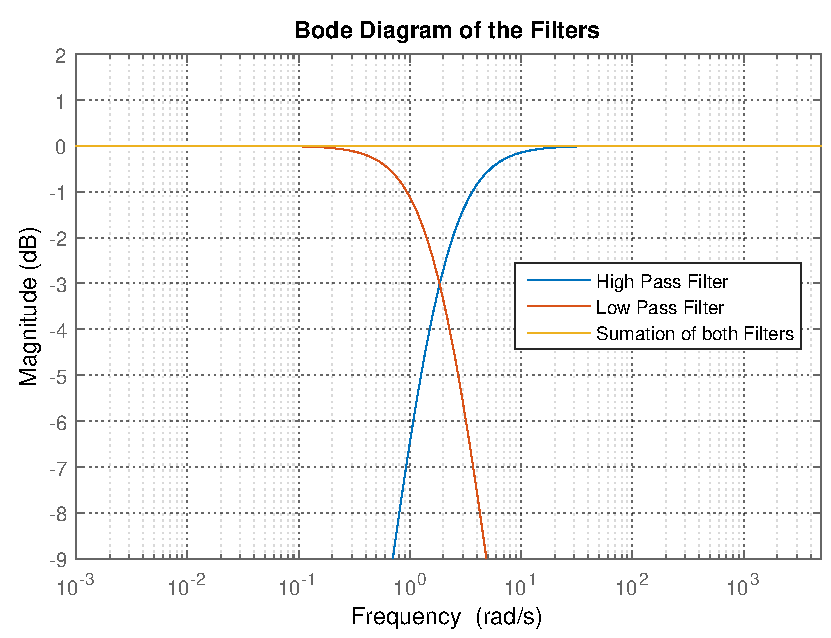
\includegraphics[scale=0.6]{Pictures/bodeFilters.pdf}
\end{figure}
%The summation of both cut-off frequency gives a gain of 1.
\end{frame}
%%%%%%%%%%%%%%%%
%%%%%%%%%%%%%%%%
\subsection{Cut-off Frequency}
\begin{frame}{Complementary Filter}{Cut-off Frequency}
%The complementary filter compared with the data from the potentiometer.
	\begin{figure}
		\centering
		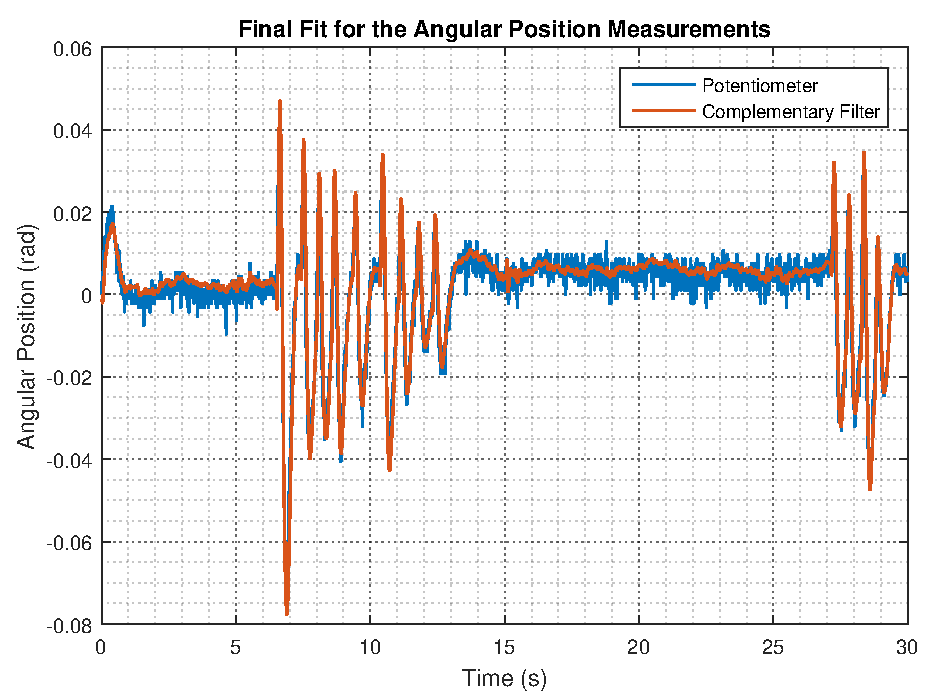
\includegraphics[scale=0.55]{Pictures/filterSensTool.pdf}
	\end{figure}
Cut-off frequency is equal to \si{1,85\ rad \cdot s^{-1}}.
%The two measurements match closely.
\end{frame}
%%%%%%%%%%%%%%%%
%%%%%%%%%%%%%%%%%%%%%%%%%%%%%%%%%% NAME %%%%%%%%%%%%%%%%%%%%%%%%%%%%%
%%%%%%%%%%%%%%%%
\section{Acceptance Test}
%%%%%%%%%%%%%%%%

%%%%%%%%%%%%%%%%
\subsection{Requirements Test 1}

\begin{frame}{Acceptance Test}{Requirements Test 1}
%- The Cubli should be able to balance starting from an unstable equilibrium position and null velocity.\linebreak
%
\begin{minipage}{\linewidth}
	\begin{minipage}{0.45\linewidth}
		\begin{figure}[H]
			\centering
			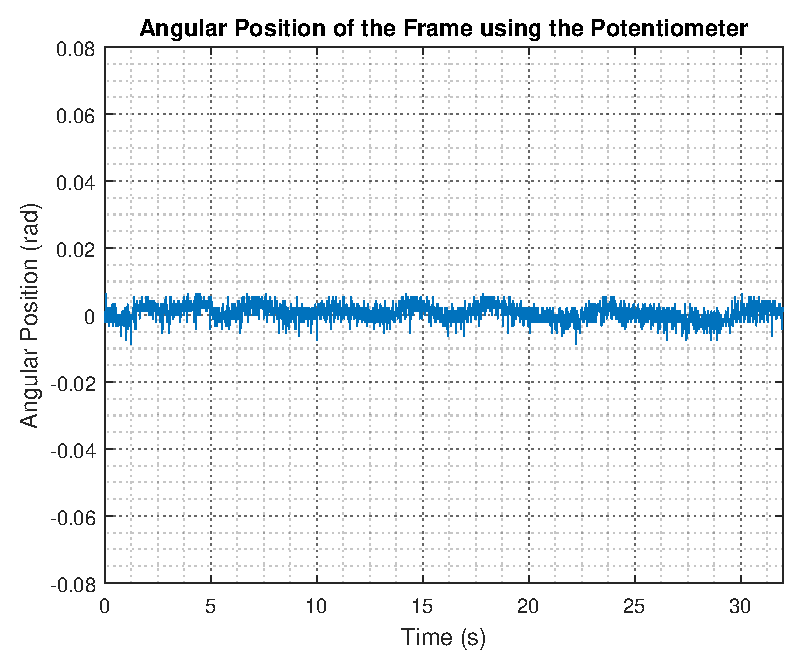
\includegraphics[scale=.345]{Pictures/testReq1}
		\end{figure}
	\end{minipage}
	\hspace{0.03\linewidth}
	\begin{minipage}{0.45\linewidth}
		\begin{figure}[H]\vspace{0mm}
			\centering
			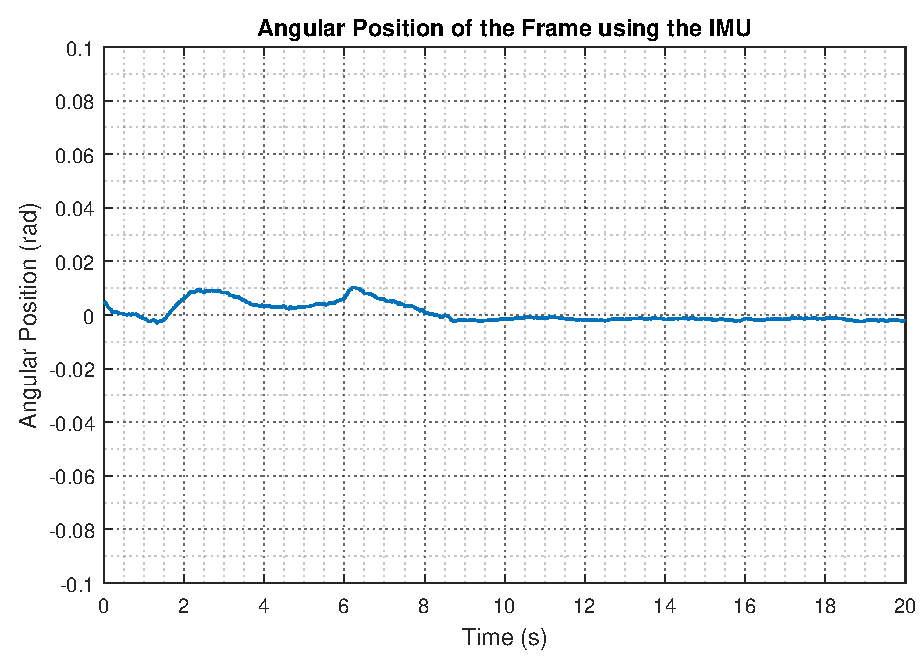
\includegraphics[scale=.345]{Pictures/testReq1_IMU}
		\end{figure}
	\end{minipage}
\end{minipage}\linebreak
%
%Angular position of the frame, when starting from equilibrium position.
%	\begin{itemize}
%		\item {Measured with the potentiometer.}
%		\item {Calculated with the complementary filter.}
%	\end{itemize}
\end{frame}
%%%%%%%%%%%%%%%%
%%%%%%%%%%%%%%%%
\subsection{Requirements Test 2}

\begin{frame}{Acceptance Test}{Requirements Test 2}
%- The prototype should be able to balance around 0 rad, even though the angle of inclination of the baseplate is changed within a reasonable range, using internally mounted sensors.
%	
\begin{figure}
	\centering
	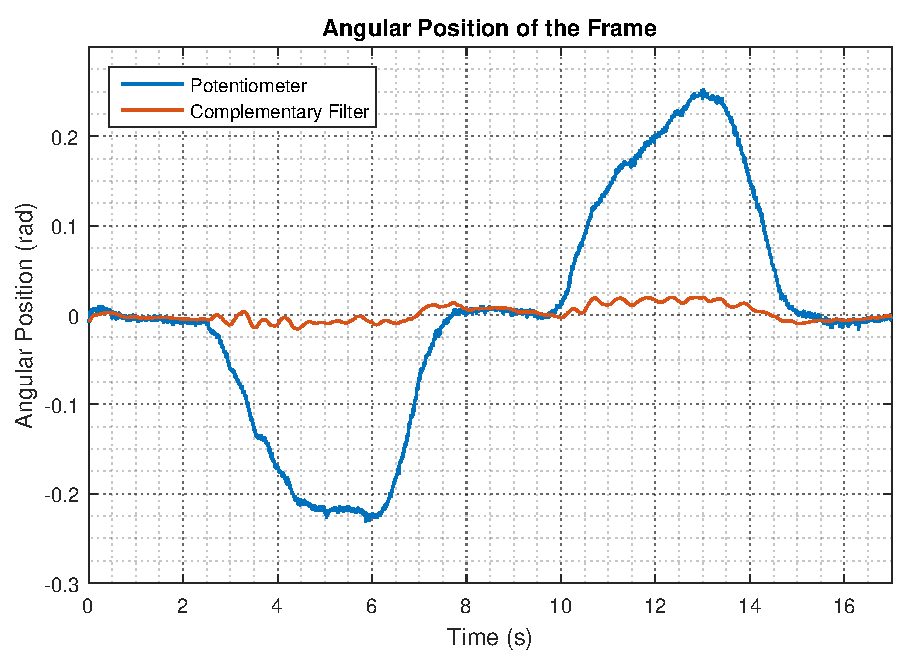
\includegraphics[scale=0.6]{Pictures/testReq2.pdf}
\end{figure}
%Position of the frame which does not depend on the angle of the baseplate.
\end{frame}
%%%%%%%%%%%%%%%%

%%%%%%%%%%%%%%%%%%%%%%%%%%%%%%%%%%% NAME %%%%%%%%%%%%%%%%%%%%%%%%%%%%%
%%%%%%%%%%%%%%%%
\section{Conclusion}
%%%%%%%%%%%%%%%%
%%%%%%%%%%%%%%%%
%\subsection{Conclusion}

\begin{frame}{Conclusion}{Cubli}
\begin{figure}
	\centering
	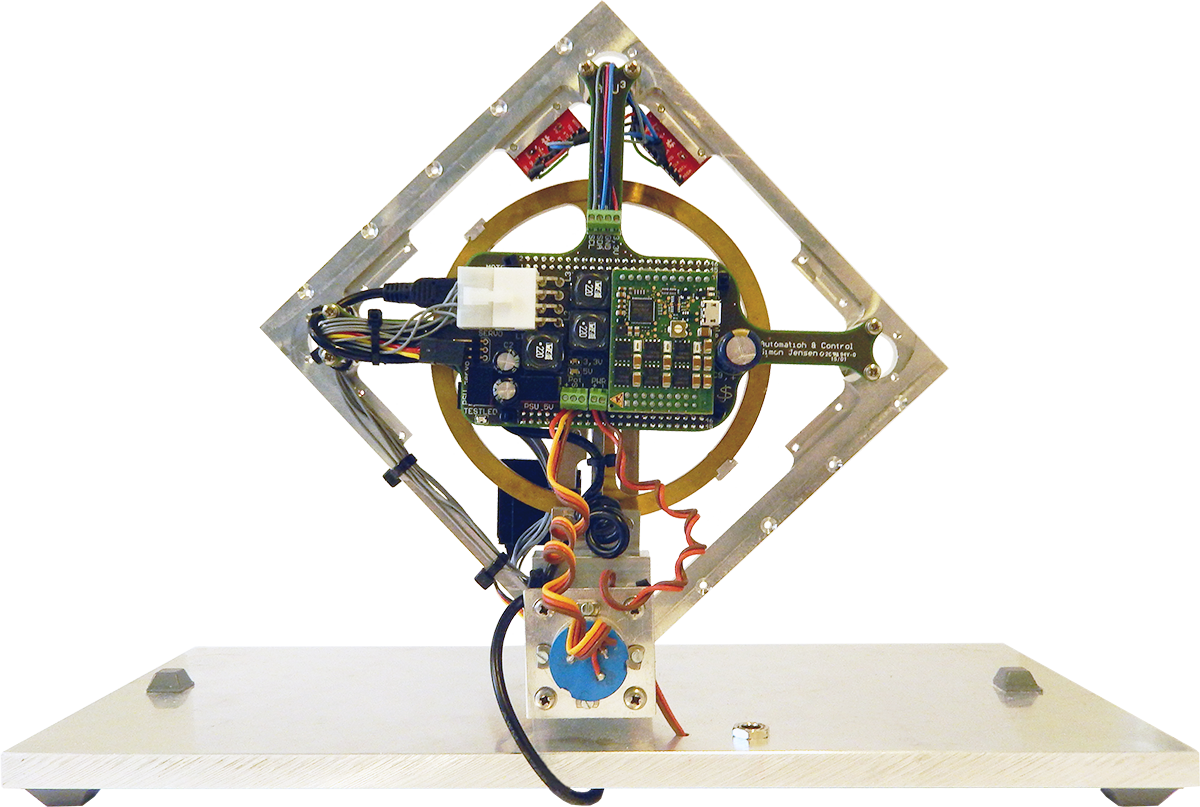
\includegraphics[scale=0.9]{Pictures/Cubli-1}
\end{figure}
%It was also a requirement to be able to:
%\begin{itemize}
%	\item {Keep it in upright position.}
%	\item {Change the angle of the baseplate.}\linebreak
%\end{itemize}
%

%	Improving the system:
%	\begin{itemize}
%		\item {Measurements of the IMU could be improved by moving the sensor.}
%		\item {Fusing Sensor data from IMU using a different filter type.}\linebreak
%	\end{itemize}
%	
%In conclusion:
%	\begin{itemize}
%		\item {The state space controller constructed has been tested successfully within the requirements.}
%	\end{itemize}
\end{frame}
%%%%%%%%%%%%%%%%
%%%%%%%%%%%%%%%%
%\subsection{Conclusion}
%
%\begin{frame}{Conclusion}{Cubli}
%	Maximum recovery angle while disturbances is applied:
%	\begin{itemize}
%		\item {The controller is capable of recovering from \si{0,08\ rad} (\si{4,58^\circ}).}
%		\item {The controller is not able to recover from greater angle due to overshoot.}\linebreak
%	\end{itemize}
%	
%	Maximum catching angle with no initial velocity of the wheel is \si{0,2024\ rad} (\si{11,59^\circ}):
%	\begin{itemize}
%		\item {The controller is capable of catching the frame when it starts from \SI{-0,17}{rad}  (\si{-9,74^\circ}).}
%		\item {The controller is not able to recover from greater angle due to overshoot.}\linebreak
%	\end{itemize}
%	It is not possible to catch and balance the system in equilibrium position from a  greater angle than \SI{-0,17}{rad}  (\si{-9,74^\circ}).\linebreak
%\end{frame}
%%%%%%%%%%%%%%%%